\documentclass[12pt,a4paper]{article}
\usepackage[a4paper,left=2cm,right=2cm,top=2cm,bottom=4cm]{geometry}
\usepackage[utf8]{inputenc}
\usepackage[T1]{fontenc}
\usepackage{amsmath}
\usepackage[ngerman]{babel}
\usepackage{amssymb}
\usepackage{float}
\usepackage{graphicx}
\usepackage{titling}

\usepackage{xcolor}
\usepackage{titlesec}



\definecolor{xsens}{RGB}{0,115,188}
\usepackage{sectsty}
%\chapterfont{\color{xsens}}  % sets colour of chapters
%\sectionfont{\color{xsens}}  % sets colour of sections
%\chapterfont{\color{xsens}}


\author{Mirco Huber}
\newcommand{\subtitle}{Reproduktion Messergebnisse}
\title{X-106 30 $\mu\varepsilon$}


%%%%%%%%%%%%%%%%%% HEADER AND FOOTER
\usepackage{fancyhdr}
\setlength\headheight{40pt}
\renewcommand{\headrulewidth}{0pt}

\lhead{\thetitle}
\rhead{
\includegraphics[height=4em]{Logos/X-SENSORS-Logo_Slogan_EN_Transparent.png}}
\rfoot{\thepage}
\cfoot{}

\fancypagestyle{plain}{%
	\setlength\headheight{40pt}
	\renewcommand{\headrulewidth}{0pt}
	\lhead{\thetitle}
	\rhead{
\includegraphics[height=4em]{Logos/X-SENSORS-Logo_Slogan_EN_Transparent.png}}
	\rfoot{\thepage}
	\cfoot{}
	
}

\fancypagestyle{empty}{%
	\fancyhf{}
}

\usepackage{subfiles}

\titleformat{\chapter}[display]
{\normalfont\huge\bfseries}{}{0pt}{\thechapter.\ }

\usepackage{nicefrac}
\usepackage{tocloft}


\pagestyle{fancy}
\begin{document}
	\thispagestyle{empty}
	\begin{titlepage}
		\begin{figure}[H]
			\centering
			
\includegraphics[width=.5\linewidth]{Logos/X-SENSORS-Logo_Slogan_EN_Transparent.png}
		\end{figure}
		\vspace*{3cm}
		\begin{center}
			\Huge {\thetitle} \\\vspace*{.5cm}
			\small {\subtitle}
		\end{center}
		\vspace{12cm}
		\hspace{.6\linewidth} 
		\begin{tabular}{l}	
			\small{\theauthor} \\[.5pt]  
			\small{X-Sensors AG} \\ 
			\small{Landenbergerstrasse 13} \\
			\small{CH-8253 Diessenhofen} \\ [.5cm] 	
			\today
		\end{tabular}
	\end{titlepage}

	\newpage
	\setcounter{page}{1}
	\pagenumbering{arabic} % A-Z Seiten (werden ausgeblendet), geht nur um PDF
	\pagestyle{fancy}
	
	
	
	%%%%%%%%%%%%%%%%%%%%%%%%%%%
	\section{Testaufbau}
	Da der Sensor hochempfindlich ist, hat bereits eine Umpositionierung auf einer ebenen Tischfläche einen Einfluss auf das Sensorsignal. Da der Sensor in einer Anwendung festgeschraubt ist, kommen diese Effekte nicht zum Tragen. Um den Sensor auf seine Eigenschaften wie Nullpunktstabilität, Warmlaufverhalten und \textit{Return-to-Zero} zu untersuchen, wird der Sensor für alle durchgeführten Messungen mit einer Schraubzwinge auf eine Tischplatte aufgespannt. Die Aufspannsituation ist in der untenstehenden Abbildung visualisiert.
	\begin{figure}[H]
		\centering
		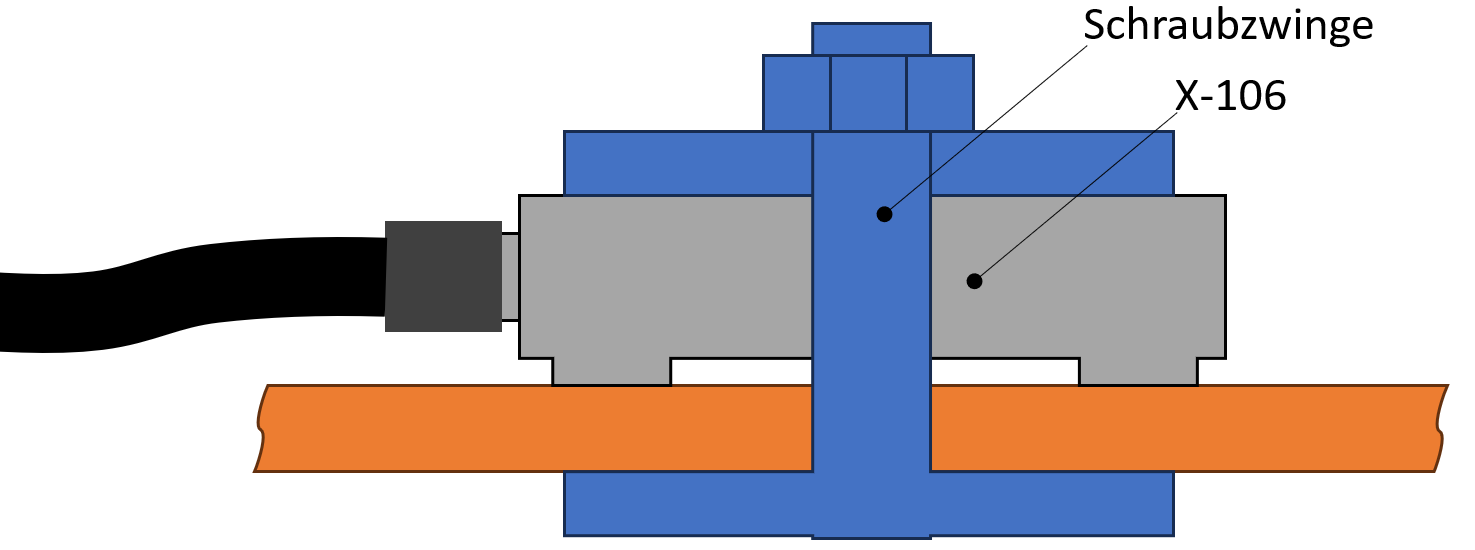
\includegraphics[width=1\linewidth]{Bilder/Aufbau}
		\caption{Testaufbau für sämtliche Messungen}
		\label{fig:aufbau}
	\end{figure}
	
	\section{Warmlaufverhalten}
	Das Warmlaufverhalten wurde mittels vergossenem Sensor (gleicher Stand wie letzte Lieferung) reproduziert. Hierfür wurde der Sensor mit einer Schraubzwinge auf eine Tischplatte aufgespannt, da geringste Berührungen/Verschiebungen bei dieser Sensorempfindlichkeit das Ausgangssignal stark beeinflussen. Durch die Aufspannung ist die Situation vergleichbar mit der Einbausituation.\\
	Die Messung wurde mehrfach durchgeführt. Der Sensor wurde hierfür für einige Messungen abgekühlt (auf eine Grundkörper-Temperatur von 12.5$^\circ$C, gemessen mit FLUKE Kontaktlos-Thermometer) und für die übrigen Messungen von einer Starttemperatur von RT 22.5$^\circ$C gestartet.
	\begin{figure}[H]
		\centering
		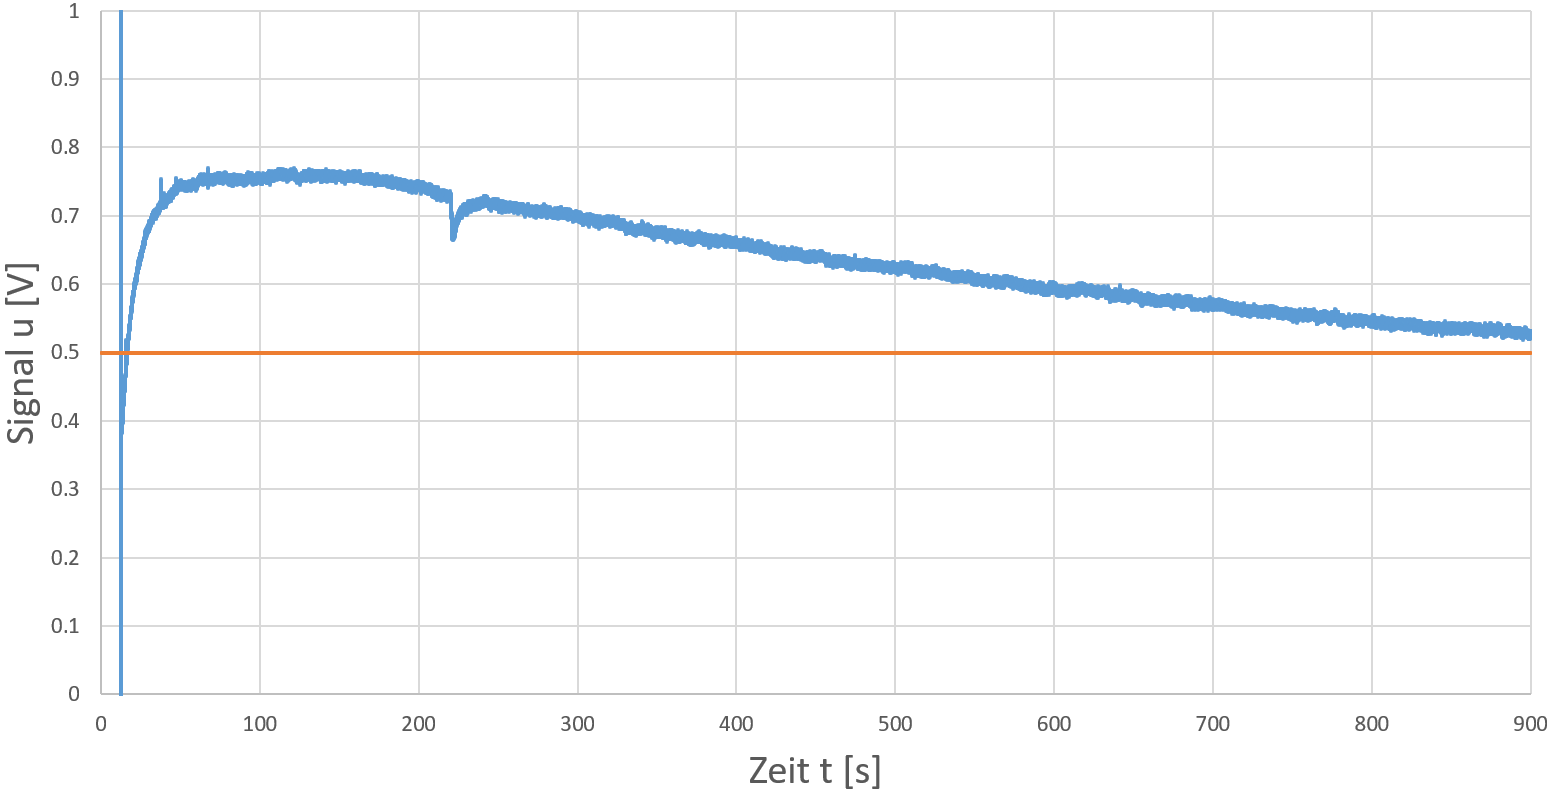
\includegraphics[width=.8\linewidth]{Bilder/warmup001}
		\caption[Warmlaufverhalten Raumtemperatur]{Warmlaufverhalten Raumtemperatur}
		\label{fig:warmup001}
	\end{figure}
	\begin{figure}[H]
		\centering
		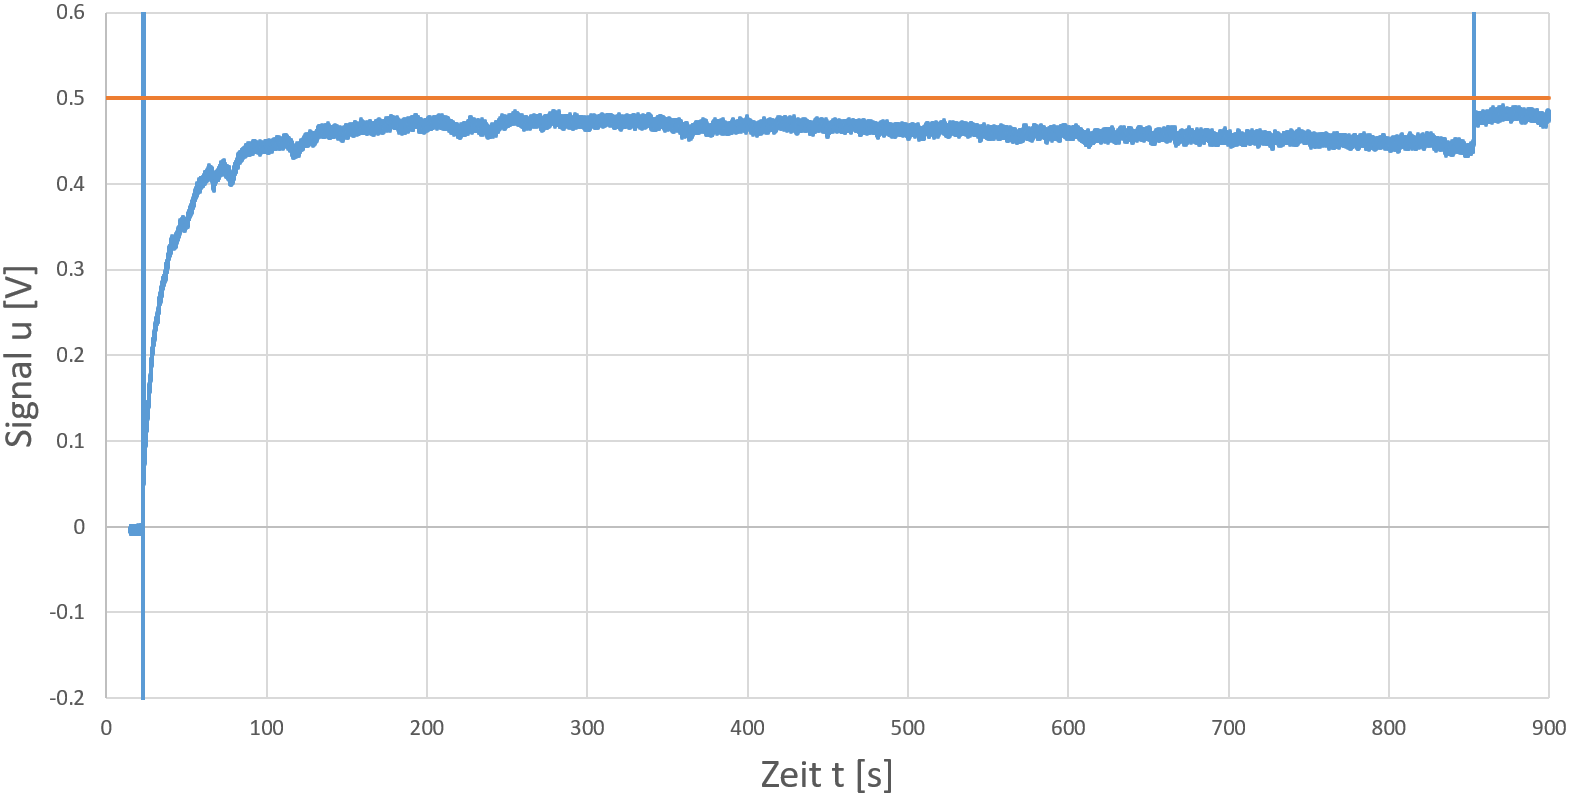
\includegraphics[width=.8\linewidth]{Bilder/warmup002}
		\caption[Warmlaufverhalten Vorgekühlt (12.5$^{\circ}$C)]{Warmlaufverhalten Vorgekühlt (12.5$^{\circ}$C)}
		\label{fig:warmup002}
	\end{figure}\noindent
	Die Messungen zeigen einen Signaldrift von $\approx 0.4$V über einen Zeitraum von 15min, was vergeichbar mit dem Serienmodell von Sumitomo ist. Die Beobachtung, dass das Signal um 2.8V driftet, konnte nicht reproduziert werden.

	\section{Handbelastungen}
	Der Sensor wurde in aufgespanntem Zustand mehrfach von Hand belastet. Die Messung zeigt eine (für diesen simplen Testaufbau) stabile Return-to-Zero-Charakteristik. Der Sensor wies nach dem Aufspannen ein Signal von rund 0.2V auf und wurde in der Messung nach 5 Sekunden tariert.
	\begin{figure}[H]
		\centering
		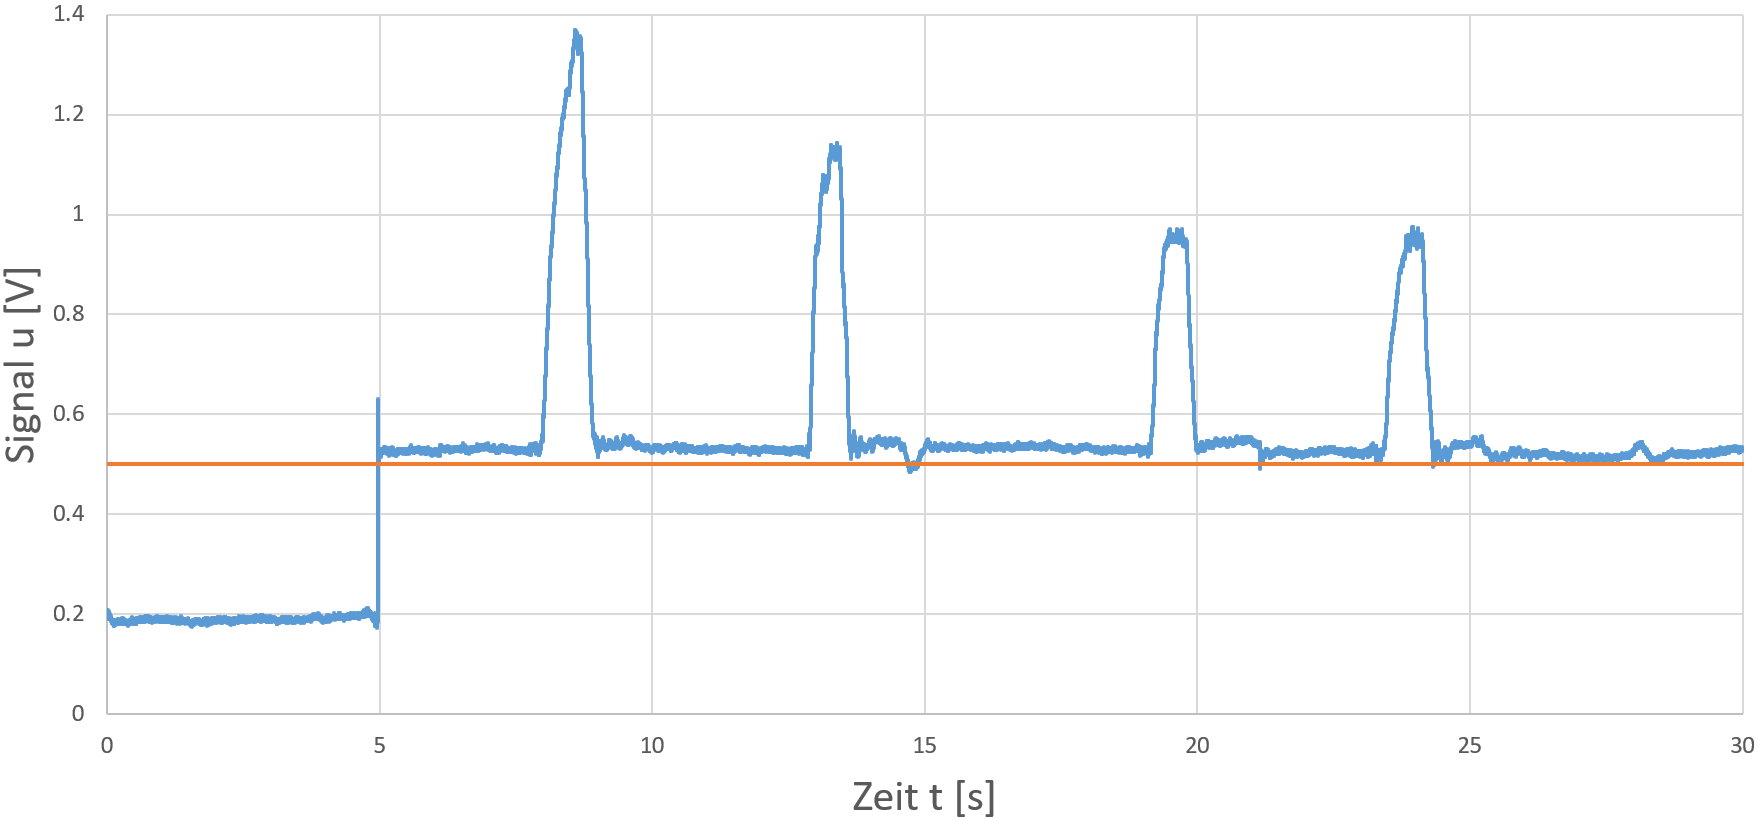
\includegraphics[width=1\linewidth]{Bilder/warmup003}
		\caption{Sensorreaktion auf Handbelastung}
		\label{fig:warmup003}
	\end{figure}
	\section{Tarieroffset / Residuum}
	Mit der aktuellen Hardware kann nach der Tarierung ein Offset / Residuum von $\pm 0.03$V resultieren, was der Auflösung des DA-Wandlers geschuldet ist. Dieser Effekt kommt zum tragen, da bisherige Anwendungen einer kleineren Verstärkung bedurften und die Auflösung des DA-Wandlers hinreichend genau war. In der kommenden Redesign-Iteration wird die Auflösung erhöht, womit das Residuum deutlich kleiner wird.
	\section{Tarierverhalten: Signal während Tarasignal \textit{HIGH}}
	Die Hardware des X-106 hat einen rein analogen Signalpfad, damit die Latenz so tief wie möglich ist. Es wird lediglich digital tariert, indem mittels DA-Wandler dem Analogsignal ein Offset zugewiesen wird (anders als die bisherige Serienlösung von Sumitomo). Die Tarierlogik kann aber ebenfalls so angepasst werden, dass während anstehendem Tariersignal (Tarasignal HIGH)  das Ausgangssignal stabil auf \textit{Living Zero} von 0.5V geregelt wird. Dies wird ebenfalls mit der kommenden Redesign-Iteration verbessert.
\end{document}